% Preamble
\documentclass[12pt]{article}

% Packages
\usepackage[a4paper, includefoot,
  left=3cm, right=1.5cm,
  top=2cm, bottom=2cm,
headsep=1cm, footskip=1cm]{geometry}
\usepackage{amsmath}
\usepackage{amssymb}
\usepackage[T2A]{fontenc}
\usepackage[utf8]{inputenc}
\usepackage[english, russian]{babel}
\usepackage{stmaryrd}
\usepackage{pdfpages}
\usepackage{graphicx}
\usepackage{wrapfig}
\usepackage{amsthm}
\usepackage{framed}
\usepackage{xcolor}
\usepackage{color}
\usepackage[unicode]{hyperref}

\hypersetup{
  colorlinks=true,
  linkcolor=black,
  urlcolor=blue,
}

%new calligraphic font for subspaces 
\usepackage{euscript}
\newcommand{\cA}{\EuScript{A}}
\newcommand{\cB}{\EuScript{B}}
\newcommand{\cC}{\EuScript{C}}
\newcommand{\cD}{\EuScript{D}}
\newcommand{\cE}{\EuScript{E}}
\newcommand{\cF}{\EuScript{F}}
\newcommand{\cG}{\EuScript{G}}
\newcommand{\cH}{\EuScript{H}}
\newcommand{\cI}{\EuScript{I}}
\newcommand{\cJ}{\EuScript{J}}
\newcommand{\cK}{\EuScript{K}}
\newcommand{\cL}{\EuScript{L}}
\newcommand{\cM}{\EuScript{M}}
\newcommand{\cN}{\EuScript{N}}
\newcommand{\cO}{\EuScript{O}}
\newcommand{\cP}{\EuScript{P}}
\newcommand{\cQ}{\EuScript{Q}}
\newcommand{\cR}{\EuScript{R}}
\newcommand{\cS}{\EuScript{S}}
\newcommand{\cT}{\EuScript{T}}
\newcommand{\cU}{\EuScript{U}}
\newcommand{\cV}{\EuScript{V}}
\newcommand{\cW}{\EuScript{W}}
\newcommand{\cX}{\EuScript{X}}
\newcommand{\cY}{\EuScript{Y}}
\newcommand{\cZ}{\EuScript{Z}}

%font for text indices like transposition X^\mathrm{T}
\newcommand{\rmA}{\mathrm{A}}
\newcommand{\rmB}{\mathrm{B}}
\newcommand{\rmC}{\mathrm{C}}
\newcommand{\rmD}{\mathrm{D}}
\newcommand{\rmE}{\mathrm{E}}
\newcommand{\rmF}{\mathrm{F}}
\newcommand{\rmG}{\mathrm{G}}
\newcommand{\rmH}{\mathrm{H}}
\newcommand{\rmI}{\mathrm{I}}
\newcommand{\rmJ}{\mathrm{J}}
\newcommand{\rmK}{\mathrm{K}}
\newcommand{\rmL}{\mathrm{L}}
\newcommand{\rmM}{\mathrm{M}}
\newcommand{\rmN}{\mathrm{N}}
\newcommand{\rmO}{\mathrm{O}}
\newcommand{\rmP}{\mathrm{P}}
\newcommand{\rmQ}{\mathrm{Q}}
\newcommand{\rmR}{\mathrm{R}}
\newcommand{\rmS}{\mathrm{S}}
\newcommand{\rmT}{\mathrm{T}}
\newcommand{\rmU}{\mathrm{U}}
\newcommand{\rmV}{\mathrm{V}}
\newcommand{\rmW}{\mathrm{W}}
\newcommand{\rmX}{\mathrm{X}}
\newcommand{\rmY}{\mathrm{Y}}
\newcommand{\rmZ}{\mathrm{Z}}

%tt font for time series
\newcommand{\tA}{\mathsf{A}}
\newcommand{\tB}{\mathsf{B}}
\newcommand{\tC}{\mathsf{C}}
\newcommand{\tD}{\mathsf{D}}
\newcommand{\tE}{\mathsf{E}}
\newcommand{\tF}{\mathsf{F}}
\newcommand{\tG}{\mathsf{G}}
\newcommand{\tH}{\mathsf{H}}
\newcommand{\tI}{\mathsf{I}}
\newcommand{\tJ}{\mathsf{J}}
\newcommand{\tK}{\mathsf{K}}
\newcommand{\tL}{\mathsf{L}}
\newcommand{\tM}{\mathsf{M}}
\newcommand{\tN}{\mathsf{N}}
\newcommand{\tO}{\mathsf{O}}
\newcommand{\tP}{\mathsf{P}}
\newcommand{\tQ}{\mathsf{Q}}
\newcommand{\tR}{\mathsf{R}}
\newcommand{\tS}{\mathsf{S}}
\newcommand{\tT}{\mathsf{T}}
\newcommand{\tU}{\mathsf{U}}
\newcommand{\tV}{\mathsf{V}}
\newcommand{\tW}{\mathsf{W}}
\newcommand{\tX}{\mathsf{X}}
\newcommand{\tY}{\mathsf{Y}}
\newcommand{\tZ}{\mathsf{Z}}

%bf font for matrices
\newcommand{\bfA}{\mathbf{A}}
\newcommand{\bfB}{\mathbf{B}}
\newcommand{\bfC}{\mathbf{C}}
\newcommand{\bfD}{\mathbf{D}}
\newcommand{\bfE}{\mathbf{E}}
\newcommand{\bfF}{\mathbf{F}}
\newcommand{\bfG}{\mathbf{G}}
\newcommand{\bfH}{\mathbf{H}}
\newcommand{\bfI}{\mathbf{I}}
\newcommand{\bfJ}{\mathbf{J}}
\newcommand{\bfK}{\mathbf{K}}
\newcommand{\bfL}{\mathbf{L}}
\newcommand{\bfM}{\mathbf{M}}
\newcommand{\bfN}{\mathbf{N}}
\newcommand{\bfO}{\mathbf{O}}
\newcommand{\bfP}{\mathbf{P}}
\newcommand{\bfQ}{\mathbf{Q}}
\newcommand{\bfR}{\mathbf{R}}
\newcommand{\bfS}{\mathbf{S}}
\newcommand{\bfT}{\mathbf{T}}
\newcommand{\bfU}{\mathbf{U}}
\newcommand{\bfV}{\mathbf{V}}
\newcommand{\bfW}{\mathbf{W}}
\newcommand{\bfX}{\mathbf{X}}
\newcommand{\bfY}{\mathbf{Y}}
\newcommand{\bfZ}{\mathbf{Z}}

%bb font for standard spaces and expectation
\newcommand{\bbA}{\mathbb{A}}
\newcommand{\bbB}{\mathbb{B}}
\newcommand{\bbC}{\mathbb{C}}
\newcommand{\bbD}{\mathbb{D}}
\newcommand{\bbE}{\mathbb{E}}
\newcommand{\bbF}{\mathbb{F}}
\newcommand{\bbG}{\mathbb{G}}
\newcommand{\bbH}{\mathbb{H}}
\newcommand{\bbI}{\mathbb{I}}
\newcommand{\bbJ}{\mathbb{J}}
\newcommand{\bbK}{\mathbb{K}}
\newcommand{\bbL}{\mathbb{L}}
\newcommand{\bbM}{\mathbb{M}}
\newcommand{\bbN}{\mathbb{N}}
\newcommand{\bbO}{\mathbb{O}}
\newcommand{\bbP}{\mathbb{P}}
\newcommand{\bbQ}{\mathbb{Q}}
\newcommand{\bbR}{\mathbb{R}}
\newcommand{\bbS}{\mathbb{S}}
\newcommand{\bbT}{\mathbb{T}}
\newcommand{\bbU}{\mathbb{U}}
\newcommand{\bbV}{\mathbb{V}}
\newcommand{\bbW}{\mathbb{W}}
\newcommand{\bbX}{\mathbb{X}}
\newcommand{\bbY}{\mathbb{Y}}
\newcommand{\bbZ}{\mathbb{Z}}

%got font for any case
\newcommand{\gA}{\mathfrak{A}}
\newcommand{\gB}{\mathfrak{B}}
\newcommand{\gC}{\mathfrak{C}}
\newcommand{\gD}{\mathfrak{D}}
\newcommand{\gE}{\mathfrak{E}}
\newcommand{\gF}{\mathfrak{F}}
\newcommand{\gG}{\mathfrak{G}}
\newcommand{\gH}{\mathfrak{H}}
\newcommand{\gI}{\mathfrak{I}}
\newcommand{\gJ}{\mathfrak{J}}
\newcommand{\gK}{\mathfrak{K}}
\newcommand{\gL}{\mathfrak{L}}
\newcommand{\gM}{\mathfrak{M}}
\newcommand{\gN}{\mathfrak{N}}
\newcommand{\gO}{\mathfrak{O}}
\newcommand{\gP}{\mathfrak{P}}
\newcommand{\gQ}{\mathfrak{Q}}
\newcommand{\gR}{\mathfrak{R}}
\newcommand{\gS}{\mathfrak{S}}
\newcommand{\gT}{\mathfrak{T}}
\newcommand{\gU}{\mathfrak{U}}
\newcommand{\gV}{\mathfrak{V}}
\newcommand{\gW}{\mathfrak{W}}
\newcommand{\gX}{\mathfrak{X}}
\newcommand{\gY}{\mathfrak{Y}}
\newcommand{\gZ}{\mathfrak{Z}}

%old calligraphic font
\newcommand{\calA}{\mathcal{A}}
\newcommand{\calB}{\mathcal{B}}
\newcommand{\calC}{\mathcal{C}}
\newcommand{\calD}{\mathcal{D}}
\newcommand{\calE}{\mathcal{E}}
\newcommand{\calF}{\mathcal{F}}
\newcommand{\calG}{\mathcal{G}}
\newcommand{\calH}{\mathcal{H}}
\newcommand{\calI}{\mathcal{I}}
\newcommand{\calJ}{\mathcal{J}}
\newcommand{\calK}{\mathcal{K}}
\newcommand{\calL}{\mathcal{L}}
\newcommand{\calM}{\mathcal{M}}
\newcommand{\calN}{\mathcal{N}}
\newcommand{\calO}{\mathcal{O}}
\newcommand{\calP}{\mathcal{P}}
\newcommand{\calQ}{\mathcal{Q}}
\newcommand{\calR}{\mathcal{R}}
\newcommand{\calS}{\mathcal{S}}
\newcommand{\calT}{\mathcal{T}}
\newcommand{\calU}{\mathcal{U}}
\newcommand{\calV}{\mathcal{V}}
\newcommand{\calW}{\mathcal{W}}
\newcommand{\calX}{\mathcal{X}}
\newcommand{\calY}{\mathcal{Y}}
\newcommand{\calZ}{\mathcal{Z}}


\setcounter{tocdepth}{2}
\graphicspath{{../img}}

\theoremstyle{plain}
\newtheorem{statement}{Утверждение}[section]
\newtheorem{theorem}{Теорема}

\theoremstyle{definition}
\newtheorem{definition}{Определение}[section]
\newtheorem{property}{Свойство}[section]
\newtheorem{example}{Пример}[section]
\newtheorem*{corollary}{Следствие}

\theoremstyle{remark}
\newtheorem{remark}{Замечание}[section]

\newcommand{\HOSVD}{\emph{HOSVD}}
\newcommand{\HOOI}{\emph{HOOI}}
\newcommand{\TSVD}{\emph{TSVD}}
\newcommand{\CPD}{\emph{CPD}}

\DeclareEmphSequence{\bfseries}

\begin{document}
\title{Обзор литературы по Tensor SSA}
\date{}
\author{}
\maketitle
\section{Статьи с теорией тензорных разложений}
\subsection{\href{https://doi.org/10.1137/s0895479896305696}
{A Multilinear Singular Value Decomposition}}\label{DeLathauwer2000}
Базовая теория
по \HOSVD{} (определения, свойства).

\subsection{\href{https://doi.org/10.1137/s0895479898346995}{On the Best
    Rank-1 and Rank-\texorpdfstring{$(R_1 ,R_2 ,. . .,R_N)$}{(R1, R2,
..., RN)} Approximation of Higher-Order Tensors}}\label{DeLathauwer2000a}
Про наилучшее приближение тензора
меньшими рангами, описание алгоритма \HOOI{}, некоторые его свойства.

\subsection{\href{https://doi.org/10.1109/TIT.2018.2841377}{Tensor SVD:
Statistical and Computational Limits}}
Рассматривается
точность приближения \HOOI{} произвольного тензора по его
зашумлённому варианту при различных случаях отношения минимального
сингулярного числа тензора к уровню шума (SNR).

\subsection{
  \href{https://doi.org/10.1016/j.laa.2010.09.020}{Factorization
  strategies for third-order tensors} и
  \href{https://doi.org/10.1137/110837711}{Third-Order
    Tensors as Operators on Matrices: A Theoretical and Compu\-tational
Framework with Applications in Imaging}}\label{Kilmer2011}
В основном теория по
трёхмерным тензорам,
вводится определение \TSVD{} и его свойства.

\section{Tensor SSA с использованием HOSVD или HOOI}
\subsection{\href{https://doi.org/10.1002/nla.453}{Exponential data
    fitting using multilinear algebra: the single-channel and
multi-channel case}}\label{Papy2005}
Рассматривается задача оценки параметров комплексного сигнала
(одномерный и многомерный случаи), состоящего из
суммы комплексных экспонент с близкими частотами.
Приводится описание и обоснование тензорной модификации алгоритма
ESPRIT с применением \HOOI{}.
Проводится численное сравнение этой модификации с базовым ESPRIT.
Выявлено преимущество тензорного метода по точности оценки параметров
сигнала в смысле RRMSE, причём с увеличением уровня шума,
преимущество увеличивается.

Траекторным тензором одномерного ряда $\tX$ с параметрами $I,L: 1 < I,L < N,\,
I + L < N + 1$ считается тензор $\mathcal{X}$ размера $I\times L \times J,\,
J=N-I-L+2$, элементы которого удовлетворяют равенству
\[
  \mathcal{X}_{ilj}=x_{i+l+j-2}\qquad i\in \overline{1:I},\, l
  \in\overline{1:L},\, j \in\overline{1:J}.
\]
Визуализация на рисунке~\ref{fig:traj-hosvd-ssa}.
\begin{figure}[!ht]
  \centering
  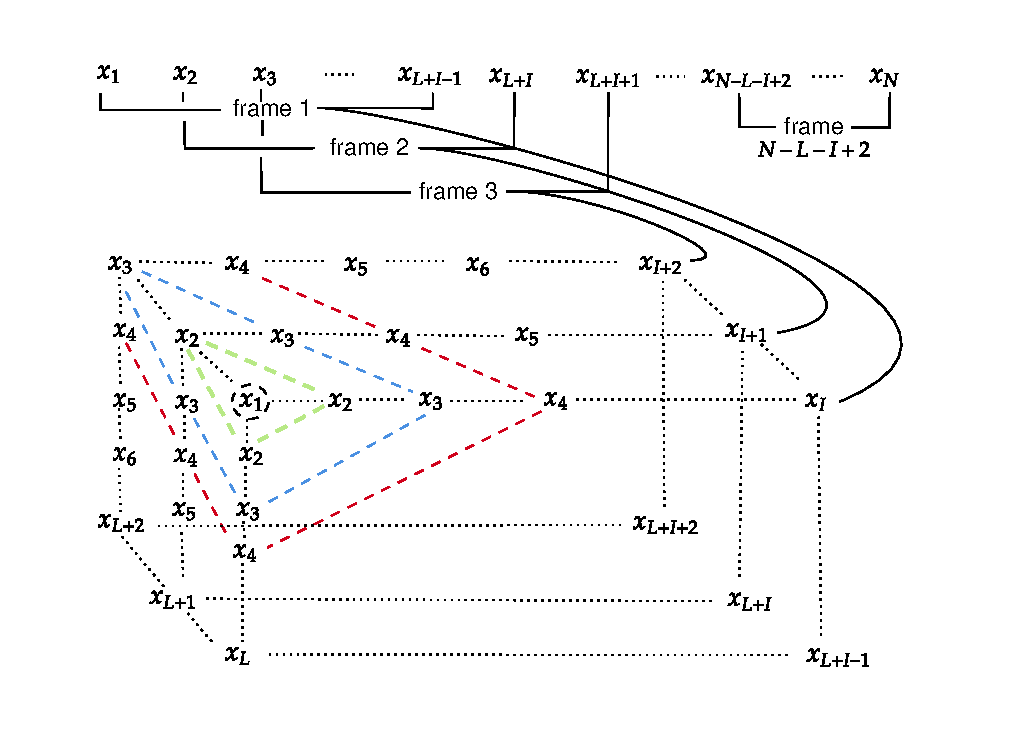
\includegraphics[width=\textwidth]{tens-injection-wide.pdf}
  \caption{Траекторный тензор одномерного ряда в
  HOSVD-SSA.}\label{fig:traj-hosvd-ssa}
\end{figure}

Траекторным тензором многомерного ряда $\tX$ с длиной окна $L:\: 1< L
< N$ считается тензор $\calX$ размерности ${L \times K \times P}$,
${K = N - L + 1}$, элементы которого удовлетворяют равенству
\[
  \calX_{lkp}=x_{l+k-1}^{(p)} \qquad l \in \overline{1:L},\, k \in
  \overline{1:K},\, p \in \overline{1:P}.
\]
Визуализация на рисунке~\ref{fig:traj-hosvd-mssa}.
\begin{figure}[!ht]
  \centering
  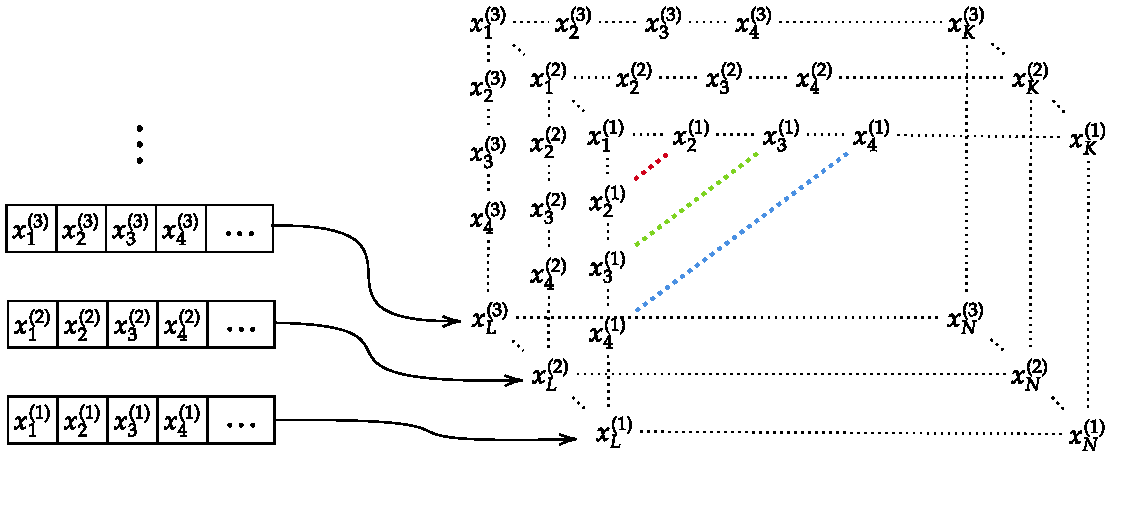
\includegraphics[width=\textwidth]{mssa_injection_new.pdf}
  \caption{Траекторный тензор многомерного ряда в HOSVD-MSSA.}
  \label{fig:traj-hosvd-mssa}
\end{figure}

Алгоритм заключается в нахождении наилучшего приближения траекторного
тензора ряда с $n$-рангами $(R, R, R)$ с помощью
алгоритма \HOOI{}.
$R$ задаётся равным числу экспонент с различными показателями входящих в сигнал.
Затем оценка строится по матрице сингулярных векторов одного из
направлений (1-го направления в одномерном случае, и 3-го в
многомерном) тем же способом, что и в базовом ESPRIT.

\pagebreak
\paragraph{Наши результаты}
\begin{enumerate}
  \item В одномерном случае оценки параметров множество длин окна,
    при которых тензорный метод даёт более точный результат, довольно мало.
    Большинство параметров длин окна в тензорном методе дают гораздо
    менее точный результат.
    Когда преимущество есть, оно невелико.
  \item В одномерном случае выделения сигнала тензорный метод не даёт
    преимущества над SSA ни при каких длинах окна.
    Наибольшей точности тензорный метод достигает при усечении
    траекторного тензора только по направлению наибольшего размера,
    особенно когда у одного из оставшихся направлений размер
    наименьший (ранг + 1).
  \item В многомерном случае оценки параметров тензорный метод точнее
    базового на одних и тех же длинах окна.
  \item В многомерном случае выделения сигнала ситуация аналогична
    задаче оценки параметров многомерного случая.
\end{enumerate}

\subsection{\href{https://doi.org/10.1002/cem.1212}{Exponential data
fitting using multilinear algebra: the decima\-tive case}}\label{Papy2009}
Рассматривается задача оценки параметров
одномерного комплексного сигнала (только одномерный случаи),
состоящего из суммы экспоненциально-модулированных гармоник с
близкими частотами.
Исследуется алгоритм HTLSDstack: модификация ESPRIT, в которой
по одномерному ряду строится $D$ прореженных рядов длины $M = N / D$ (считается,
что длина ряда $N$ делится на $D$ нацело).
Затем они считаются отдельными каналами одного многомерного ряда, и применяется
многомерный вариант ESPRIT.
Это уменьшает трудоёмкость алгоритма при небольшом уменьшении точности.
Предлагается тензорная модификация этого алгоритма: HO-HTLSDstack, в которой
к полученному многомерному ряду применяется тензорная модификация
многомерного ESPRIT из~\ref{Papy2005}.

Исходный ряд $\tX$ длины $N$ разбивается на $D$ прореженных
подрядов $\tX^{(d)}$ длины $M$ так, что $x_m^{(d)}=x_{(m-1)D + d}$.
Другими словами, в ряд с номером $d$ входит каждый $D$-й элемент
исходного ряда, начиная с $x_d$.
По полученному многомерному ряду строится траекторный тензор так же,
как в~\ref{Papy2005}.
Затем ищется наилучшее приближение этого тензора с $n$-рангами
$(R,\min(R, M), R')$, где $R$ задаётся равным числу экспонент с
различными показателями входящих в сигнал, а $R' \leqslant \min(R, D)$.
Авторы утверждают, что если частоты гармоник близки, то выбор $R' < \min(R, D)$
улучшает точность оценки параметров.

Для оценки параметров используются сингулярные векторы 1-го
направления полученного разложения аппроксимирующего тензора.

Численно показано, что тензорный вариант (HO-HTLSDstack) с выбором
$R'=1$ оказывается точнее HTLSDstack во всех тестах, причём
преимущество увеличивается с увеличением уровня шума.
Также в одном тесте HO-HTLSDstack сравнивается с базовым ESPRIT и
так же оказывается более точной.
Во всех тестах рассматривался случай близких частот.

Кроме того, авторы показывают, что метод HO-HTLSDstack меньше чем на
порядок более трудоёмкий, чем HTLSDstack, но на порядок менее
трудоёмкий, чем базовый ESPRIT.

Графики со сравнением методов по точности и трудоёмкости, приведённые
в статье, указаны на рисунке~\ref{fig:papy2009}.
\begin{figure}[!ht]
  \centering
  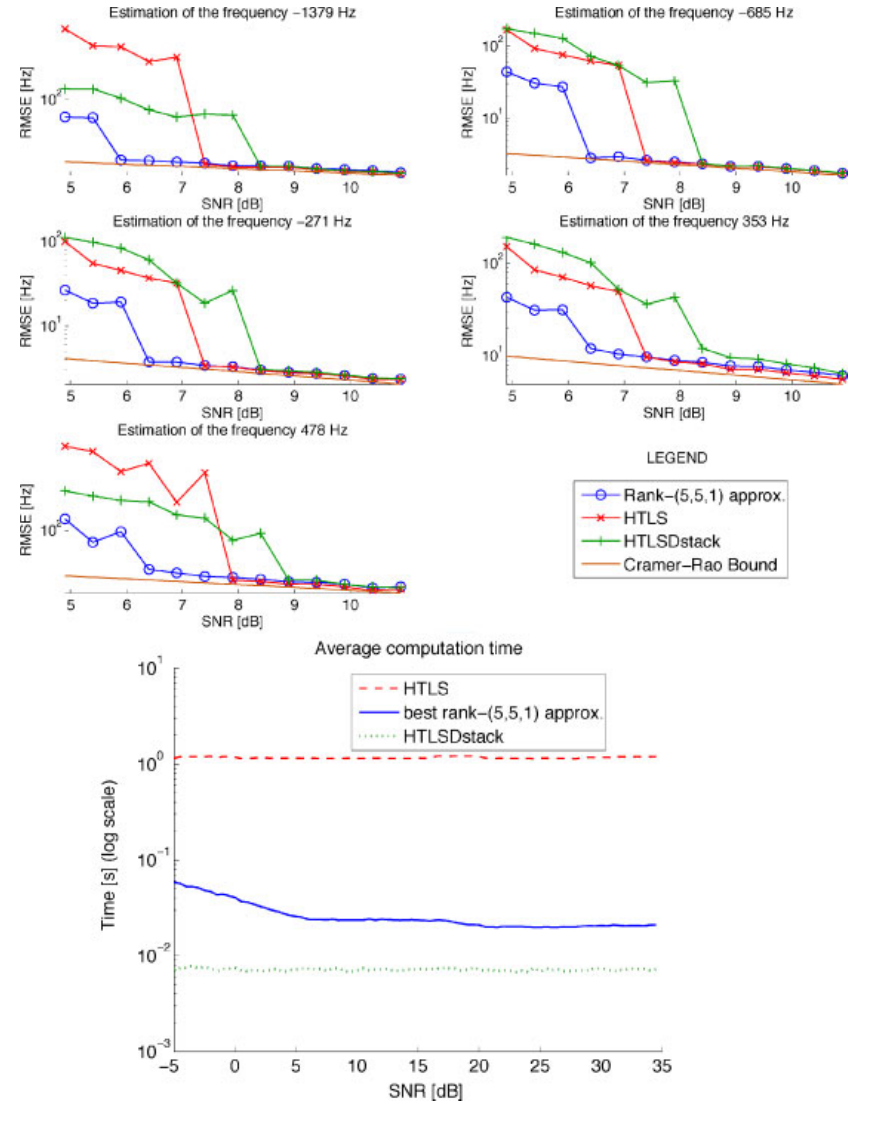
\includegraphics[height=0.8\textheight]{papy2009_figures.png}
  \caption{Сравнение HTLS (ESPRIT), HTLSDstack и HO-HTLSDstack по
  точности оценки параметров и по трудоёмкости.}
  \label{fig:papy2009}
\end{figure}

\paragraph{Наши результаты} Результаты статьи пока не проверялись.

\section{Tensor SSA с использованием \texorpdfstring{$(L_r, L_r,
1)$}{(Lr, Lr, 1)}-разложения}
\subsection{\href{https://doi.org/10.1137/100805510}{Blind Separation
    of Exponential Polynomials and the Decom\-position of a Tensor in
Rank-\texorpdfstring{$(L_r, L_r, 1)$}{(Lr, Lr, 1)} Terms}}
Приводится теоретическая информация про разложение в сумму тензоров с
$n$-рангами $(L_r, L_r, 1)$, в частности определение и условия единственности.

Рассматривается задача выделения сигнала в многомерном ряде
\[
  \bfY = \bfM \bfS + \bfN,
\]
где $\bfY$ "--- наблюдаемый ряд, $\bfS$ "--- искомый сигнал, $\bfM$
"--- коэффициенты линейных комбинаций, с которыми сигнал составляет
наблюдаемый ряд, $\bfN$ "--- шум.
Траекторный тензор ряда определяется так же, как в~\ref{Papy2005}.

Для модели, в которой сигнал составляют суммы произведений полиномов
и комплексных экспонент, доказаны условия единственности $(L_r, L_r,
1)$-разложения траекторного тензора ряда.

Метод заключается в построении траекторного тензора по ряду $\bfY$,
аппроксимации этого тензора меньшими $n$-рангами (но б\'{о}льшими, чем
$n$-ранги самого сигнала), и применении $(L_r, L_r, 1)$-разложения к
этой аппроксимации.
Далее по этому разложению можно построить оценку $\bfS$.

Проводятся численные сравнения точности выделения сигнала
предложенным методом при различных выборах параметров рангов
аппроксимации и $L_r$.
Сравнения с другими методами выделения сигнала не проводится.

\paragraph{Наши результаты} Результаты статьи пока не проверялись.

\section{Tensor SSA с использованием CPD}
\subsection{\href{https://doi.org/10.1109/tnsre.2014.2329557}{Tensor
    Based Singular Spectrum Analysis for Automatic Scoring of Sleep
EEG}}\label{Kouchaki2015}
Рассматривается задача выделения одномерного вещественного сигнала
из ряда с нестационарным шумом.

Вводится понятие траекторного тензора следующим образом: исходный
одномерный ряд делится на непересекающиеся подряды длины $l$, затем
траекторный тензор строится аналогично траекторному тензору
многомерного ряда из~\ref{Papy2005}, как если бы эти подряды были
каналами многомерного сигнала.
Предлагается алгоритм Tensor-Based SSA, основанный на применении \CPD{}
к полученному траекторному тензору ряда.

Кроме того, предлагается алгоритм TSSA-EMD, основанный на
использовании метода
EMD для адаптивной группировки компонент \CPD{}.
Метод заключается в получении \CPD{} траекторного тензора, использовании
EMD для выделения сигнала, построении траекторного тензора $\calF$
этой оценки сигнала, и решении оптимизационных задач
\[
  J(g_{ijk}) = \left\|\calF_{ijk} - \sum_{r=1}^{R}g_{ijk} a_{ir} b_{jr}
  c_{kr}\right\|^2 \to \min_{g_{ijk}}
\]
для всех $i$, $j$, $k$, где $a_{ir}$, $b_{jr}$ и $c_{jr}$ "--- компоненты CPD.
После нахождения тензора адаптивных весов $\calG=\{g_{ijk}\}$ строится оценка
траекторного тензора сигнала
\[
  \calS_{ijk} = \sum_{r=1}^{R}\calG_{ijk} a_{ir} b_{jr} c_{kr},
\]
по которому восстанавливается оценка сигнала.

Метод TSSA-EMD численно сравнивался с методами SCICA,
EEMD-ICA и SSA на моделированном ряде с нестационарным шумом (явная
формула рассматриваемого ряда в статье не приведена).
Было показано значимое преимущество TSSA-EMD над остальными
рассматриваемыми методами в смысле RMSE, причём для каждого алгоритма
рассматривался лишь один набор параметров.

Также было рассмотрено применение TSSA-EMD к реальному ряду.

\paragraph{Наши результаты}
Применение предложенного метода без адаптивной группировки с
помощью EMD давало стабильно менее точные оценки сигнала, чем базовый SSA.
Вариант TSSA-EMD не рассматривался.

\subsection{\href{https://doi.org/10.3390/app7040418}{Improved
    Tensor-Based Singular Spectrum Analysis Based on Single Channel Blind
Source Separation Algorithm and Its App\-lication to Fault Diagnosis}}
\label{Yang2017}
Рассматривается задача выделения одномерного вещественного сигнала из ряда.

Предлагается алгоритм, совпадающий с TSSA из~\ref{Kouchaki2015} (без
адаптивной группировки) во всём, кроме метода для вычисления CDP.
В~\ref{Kouchaki2015} используется ALS метод минимизации ошибки аппроксимации
\[
  \left\|\calX - \llbracket \bfA, \bfB, \bfC\rrbracket \right\|^2,
\]
где $\calX$ "--- аппроксимируемый тензор,
$\llbracket \bfA, \bfB, \bfC\rrbracket = \sum_{r=1}^{R} A_r \circ B_r
\circ C_r$.
Авторы предлагают использовать метод CP-WOPT, который заключается в построении
весового тензора $\calW$ и минимизации функционала
\[
  \left\|\calW * \calX - \calW * \llbracket \bfA, \bfB,
  \bfC\rrbracket \right\|^2,
\]
где знак $*$ "--- поэлементное умножение.
Эта модификация призвана улучшить сходимость разложения.

Кроме того предлагалось использовать алгоритм EMD-SVD-BIC для
определения числа компонент в CPD.
Этот алгоритм заключается в нахождении с помощью EMD сигнальных
компонент (IMF), построении их ковариационной матрицы, проведении SVD
этой матрицы, вычислении BIC по сингулярным числам ковариационной
матрицы при различных предположениях о числе сигнальных компонент.

Проводятся численные сравнения предложенного метода CP-WOPT TSSA с
немодифицированным TSSA из~\ref{Kouchaki2015}, Fast-ICA и EMD-ICA на
ряде не конечного ранга (пульсирующая затухающая гармоника).
Утверждается преимущество предложенного метода, но без подтверждения
какой либо метрикой (лишь визуальные подтверждения).

\paragraph{Наши результаты}
CP-WOPT метод не был применён, так как из статьи неясно по какому
принципу строится весовой тензор $\calW$.
Было проведено сравнение TSSA из~\ref{Kouchaki2015} c SSA и MSSA на
ряде предложенного в статье вида.
Оказалось, что на таком ряде TSSA выделяет сигнал точнее, чем SSA, но
менее точно, чем MSSA.
Под применением MSSA к одномерному ряду имеется в виду разделение
ряда на непересекающиеся подряды одной длины, и рассмотрение их как
каналов многомерного ряда.
\end{document}